\documentclass{article}

% cool tables
\usepackage{booktabs}
\newcommand{\ra}[1]{\renewcommand{\arraystretch}{#1}}

% images
\usepackage{graphicx}


\title{\Huge Project plan \\ 
    \normalsize  Project name: Rock Concert Audience as a Screen \\
    Project sponsor: Netlight AS \\
    Project advisor: Anh Nguyen Duc}
\author{Agnethe Soraa,
Tomas Dohnalek,
Jan Bednarik,
Milos Jovac}
\date{\today}

\begin{document}
\maketitle
\section{Project customer}
Netlight AS is a consulting company engaged in IT and management. They operates throughout Europe with offices in Stockholm, Oslo, London, Munich and Helsinki. The company was founded at 1999 and employs to 500 employes.

\section{Project background}
In order to expand audience's experience during a concert

\section{Required work}
\section{Project scope}
\section{Project architecture}
\section{Measurement of Project Effects}
\section{Planned workload}
\section{General Terms}
\section{Schedule}
\subsection{Gantt chart}

\begin{figure}[ht]
\begin{center}
    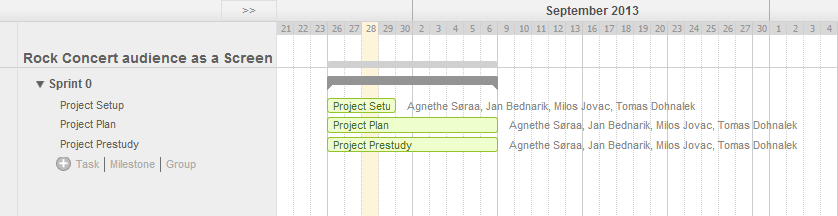
\includegraphics[scale=0.6]{images/gantt}
    \caption{Gantt Chart}
    \label{img:gantt}
\end{center}
\end{figure}

\subsection{Milestones}
\section{Risk managament}

\begin{table*}\centering \ra{1.3}
    \caption{Skills}
    \label{tab:skills}
    \vspace{2mm}
    \begin{tabular}{lcccc}
    \toprule
                                & Agnethe   & Tomas & Milos & Jan \\
    \midrule
    \textbf{Leadership                 } & 4         & 1     & 2     & 3     \\ 
    \textbf{Scrum                      } & 4         & 1     & 1     & 1     \\ 
    \textbf{Mobile software development} & 3         & 1     & 4     & 1     \\ 
    \textbf{\LaTeX                     } & 1         & 4     & 1     & 4     \\ 
    \textbf{Network programming        } & 2         & 3     & 3     & 3     \\ 
    \textbf{Image processing           } & 1         & 3     & 1     & 2     \\ 
    \textbf{Java                       } & 3         & 2     & 5     & 1     \\ 
    \textbf{C++                        } & 1         & 4     & 3     & 4     \\ 
    \textbf{Testing                    } & 1         & 4     & 2     & 3     \\
    \bottomrule
    \end{tabular}
\end{table*}


\end{document}
